\documentclass{article}
\usepackage[utf8]{inputenc}
\usepackage{blindtext}
\usepackage{multicol}
\usepackage{multirow}
\usepackage{graphicx}
\usepackage{amsmath}
\usepackage{biblatex}
\usepackage{authblk}
\usepackage{algorithm}
\usepackage{algpseudocode}
\usepackage{bbding}
\usepackage{pifont}
\usepackage{wasysym}
\usepackage{amssymb}
\usepackage{subcaption} 
\usepackage{biblatex}
\usepackage{rotating}
\usepackage{hyperref}
\usepackage{listings}
\usepackage{geometry}
\usepackage{setspace}
\usepackage{minted}
\geometry{left=1in, right=1in}

\begin{document}
\newpage
\begin{Large}
\begin{center}

\includegraphics[width=0.3\textwidth]{logo/buet.png}\\

\textbf{{\huge Assignment on Motif Search Algorithm}}
\end{center}
\textbf{Course No:} CSE463\\
\textbf{Course Title:} Introduction to Bioinformatics
\\
\\
\\
\\
\textbf{Submitted To:}\\
Dr. Muhammad Ali Nayeem\\
Assistant Professor,\\
Department of Computer Science and Engineering,\\
Bangldesh University of Engineering and Technology
\\
\\
\\
\\
\textbf{Submitted By:}\\
1905012 - Faria Binta Awal\\
1905035 - Farhan Tahmidul Karim\\
1905045 - Md. Ishrak Ahsan\\
1905046 - Niaz Rahman\\
1905050 - Riad Ahmed Anonto\\

\newpage
\tableofcontents
\newpage

\section{Data}
In bioinformatics, a \textbf{biomarker} is a measurable indicator of a biological state or condition, while \textbf{ground truth} refers to the actual, true state of a given sample or dataset. Ground truth is essential for evaluating the performance of bioinformatics methods, as it provides a reference for assessing the accuracy and reliability of the methods.\\

But we did not find any dataset with ground truth upon searching on internet.So, the whole experiment is done by using the dataset provided in in the assignment materials.

\section{Methods}
We have implemented two well-known algorithms of motif search with some modifications.
\subsection{Randomized Algorithm + Genetic Algorithm}
Genetic Algorithm (GA) solve optimization problems by mimicking the process of natural selection. Genetic Algorithm  operate by evolving a population of individual solutions over successive generations towards an optimal solution. At each step, the algorithm selects individuals from the current population as parents to produce children for the next generation. Through selection, crossover, and mutation rules, Genetic Algorithm create new generations of solutions that evolve towards better outcomes. This iterative process allows Genetic Algorithm  to address optimization problems. By generating a population of points at each iteration and selecting the best points to approach an optimal solution, Genetic Algorithm excel in exploring complex solution spaces and can converge towards global optima.

Thus, Genetic Algorithms can improve Randomized Motif Search by providing a robust and efficient framework for exploring the search space of possible motifs.This approach explores the search space of all possible starting locations of binding site motifs in a sequence, iteratively improving the population of solutions through selection, crossover, and mutation rules.
\begin{figure}[h]
    \centering
    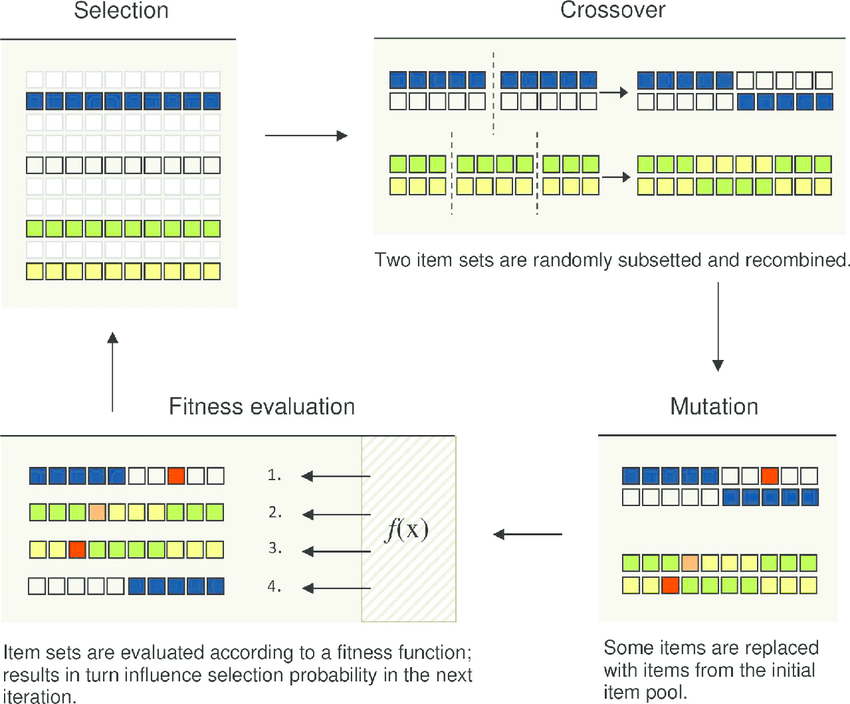
\includegraphics[width=0.8\textwidth]{methods/genetic-algorithm.png}
    \caption{Concept of Genetic Algorithm}
\end{figure}

\subsection{Gibbs Sampler + Simulated Annealing}
Simulated Annealing is a probabilistic optimization technique inspired by the annealing process in metallurgy. It is used to approximate the global optimum of a given function, particularly when dealing with large search spaces and numerous local optima.Simulated annealing starts with an initial solution and iteratively improves it by randomly perturbing it. The probability of accepting a worse solution is initially high and gradually decreases as the number of iterations increases. This approach allows the algorithm to escape local minima and converge to a global minimum. 

Thus,by incorporating Simulated Annealing into the Gibbs Sampler motif search, it becomes possible to improve the algorithm's ability to find optimal motifs by enabling it to overcome local minima and explore different regions of the search space more effectively.
\begin{figure}[h]
    \centering
    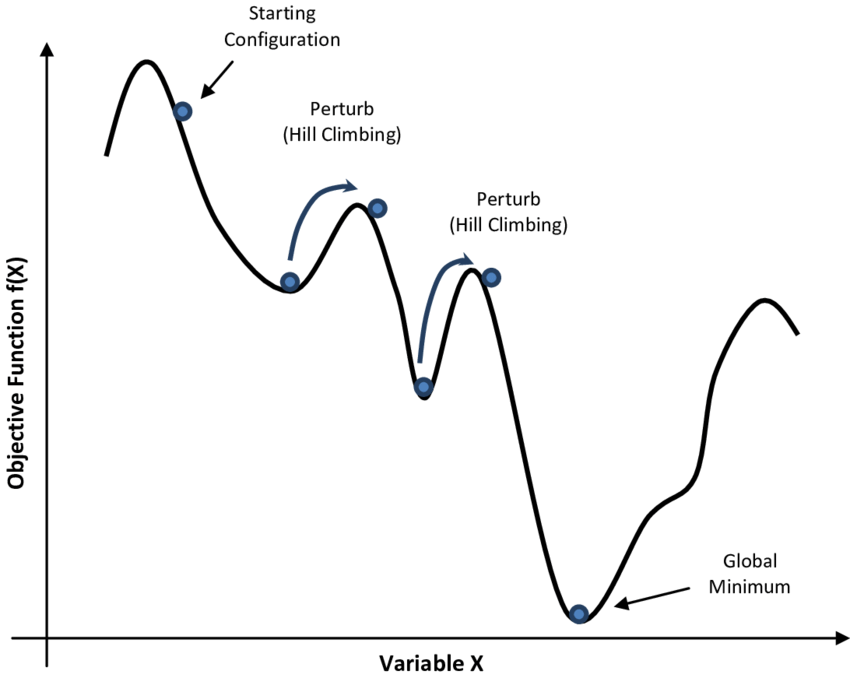
\includegraphics[width=0.8\textwidth]{methods/simulated-annealing.png}
    \caption{Concept of Simulated Annealing}
\end{figure}

\section{Software}
We have used two softwares. Both the software have online version as well as command line version.
\subsection{MEME}
Multiple EM for Motif Elicitation is referred to as MEME. In certain sequences, MEME finds new, ungapped motifs—repeated, fixed-length patterns—in the sample output obtained from the sequences. Variable-length patterns are divided into two or more distinct motifs by MEME. Motifs are represented by MEME as position-dependent letter-probability matrices, which indicate the likelihood of every possible letter at every pattern point. MEME motifs don't have any holes in them. MEME divides patterns with gaps of varying lengths into two or more distinct motifs. A set of sequences is fed into MEME, which returns as many motifs as asked. MEME automatically determines the ideal width, quantity of occurrences, and description for each motif using statistical modeling approaches.
\subsubsection{Commands to run}
\begin{minted}{bash}
$ meme sequences.fa -dna -oc . -nostatus -time 14400 -mod zoops 
 -nmotifs 3 -minw 6 -maxw 50 -objfun classic -revcomp -markov_order 0
\end{minted}

\subsubsection{Scripts to run}
\begin{minted}{bash}
for i in {1..10}; do
    echo "Running command..."
    
    meme sequences.fa -dna -oc . -nostatus -time 14400 
    -mod zoops -nmotifs ($i+5) -minw ($i+5) -maxw ($i+40) 
    -objfun classic -revcomp -markov_order 0

    mast meme.xml sequences.fa -oc . -nostatus
done
\end{minted}


\subsection{STREME}
Simple, Thorough, Rapid, Enriched Motif Elicitation is known as STREME. STREME finds recurrent, fixed-length patterns known as ungapped motifs that are either comparatively or significantly more abundant in your sequences as compared to a set of control sequences (sample output from sequences). STREME scans large sequence databases for motifs, up to 30 columns wide. One or two sets of sequences are the input for STREME. The distribution of lengths for the control and primary sequences need to be almost identical. The software shuffles the primary set to produce a control set if no control set is supplied. Using a significance threshold, the program compares each motif identified in the positive set with its representation in the control set. STREME delivers precise estimations of the statistical significance of the motifs it finds and operates at fast speed thanks to an optimization technique that makes use of a suffix tree.
\subsubsection{Commands to run}
\begin{minted}{bash}
    $ streme --verbosity 1 --oc . --dna --totallength 4000000 
    --time 14400 --minw 8 --maxw 15 --thresh 0.05 --align center 
    --p sequences.fa
\end{minted}

\subsubsection{Scripts to run}
\begin{minted}{bash}
for i in {1..10}; do
    echo "Running command..."
    
    streme --verbosity 1 --oc . --dna --totallength 4000000 
    --time 14400 --minw ($i+5) --maxw ($i+40) --thresh ($i/100) 
    --align center --p sequences.fa

    mast streme.xml sequences.fa -oc . -nostatus
done
\end{minted}

\section{Results}
\subsection{Experiment Configuration}
Ten sequences with lengths totaling 1500 may be found in the first data collection, designated with the code hm03r, for which the hm abbreviation derives from the human language. The yeast contains 7 and 11 sequences in the second and third data sets associated with the yst04r and yst08r, for which the yst acronym is derived. The sequences in yst04r and yst08r have lengths of 1000. \\

We have varied the length of motif for both of our algorithm. Genetic Algorithm uses two extra parameter like mutation rate and population size while Simulated Annealing uses one extra parameter called temperature. We have also varied these parameters.\\

MEME and STREME uses different output parameter.So we will use one of them. We will consider information content(simple modification by us) as score for MEME and will consider matches per sequence (simple modification by us) as score for STREME.\\

We have also calculated the time to find the motif for each of our algorithm.It will indicate how fast our algorithms compared to the tools.\\

Finally, we will compare based on two parameters - Score and Time.

\subsection{Comparison}
We will consider \textcolor{blue}{Randomized Algorithm + Genetic Algorithm} as \textcolor{blue}{Method1} and \textcolor{blue}{Gibbs Sampler + Simulated Annealing} as \textcolor{blue}{Method2}.
\newpage
\subsubsection{Method1 vs MEME}

\begin{table}[h]
\centering
\caption{hm03}
\begin{tabular}{|c|cc|cc|}
\hline
\multirow{2}{*}{\begin{tabular}[c]{@{}c@{}}Motif \\ Length\end{tabular}} & \multicolumn{2}{c|}{Method1}                                                                                                               & \multicolumn{2}{c|}{MEME}                                                                                                               \\ \cline{2-5} 
                                                                         & \multicolumn{1}{c|}{\begin{tabular}[c]{@{}c@{}}Average\\ Score\end{tabular}} & \begin{tabular}[c]{@{}c@{}}Time\\ (in seconds)\end{tabular} & \multicolumn{1}{c|}{\begin{tabular}[c]{@{}c@{}}Average\\ Score\end{tabular}} & \begin{tabular}[c]{@{}c@{}}Time\\ (in seconds)\end{tabular} \\ \hline
9                                                                        & \multicolumn{1}{c|}{12.2}                                                    & 30.06                                                       & \multicolumn{1}{c|}{11.5}                                                    & 25.23                                                       \\ \hline
11                                                                       & \multicolumn{1}{c|}{15.5}                                                    & 33.11                                                       & \multicolumn{1}{c|}{15.2}                                                    & 27.25                                                       \\ \hline
13                                                                       & \multicolumn{1}{c|}{19.1}                                                    & 37.19                                                       & \multicolumn{1}{c|}{19.1}                                                    & 30.37                                                       \\ \hline
19                                                                       & \multicolumn{1}{c|}{23.9}                                                    & 43.10                                                       & \multicolumn{1}{c|}{22.3}                                                    & 36.29                                                       \\ \hline
22                                                                       & \multicolumn{1}{c|}{30.7}                                                    & 45.39                                                       & \multicolumn{1}{c|}{27.8}                                                    & 39.58                                                       \\ \hline
\end{tabular}
\end{table}

\begin{table}[h]
\centering
\caption{yst04r}
\begin{tabular}{|c|cc|cc|}
\hline
\multirow{2}{*}{\begin{tabular}[c]{@{}c@{}}Motif \\ Length\end{tabular}} & \multicolumn{2}{c|}{Method1}                                                                                                               & \multicolumn{2}{c|}{MEME}                                                                                                               \\ \cline{2-5} 
                                                                         & \multicolumn{1}{c|}{\begin{tabular}[c]{@{}c@{}}Average\\ Score\end{tabular}} & \begin{tabular}[c]{@{}c@{}}Time\\ (in seconds)\end{tabular} & \multicolumn{1}{c|}{\begin{tabular}[c]{@{}c@{}}Average\\ Score\end{tabular}} & \begin{tabular}[c]{@{}c@{}}Time\\ (in seconds)\end{tabular} \\ \hline
9                                                                        & \multicolumn{1}{c|}{10.2}                                                    & 31.06                                                       & \multicolumn{1}{c|}{9.5}                                                    & 25.23                                                       \\ \hline
11                                                                       & \multicolumn{1}{c|}{13.5}                                                    & 33.11                                                       & \multicolumn{1}{c|}{11.2}                                                    & 28.25                                                       \\ \hline
13                                                                       & \multicolumn{1}{c|}{15.1}                                                    & 35.19                                                       & \multicolumn{1}{c|}{14.1}                                                    & 30.37                                                       \\ \hline
19                                                                       & \multicolumn{1}{c|}{22.9}                                                    & 40.10                                                       & \multicolumn{1}{c|}{20.3}                                                    & 35.39                                                       \\ \hline
22                                                                       & \multicolumn{1}{c|}{30.7}                                                    & 43.39                                                       & \multicolumn{1}{c|}{28.8}                                                    & 39.58                                                       \\ \hline
\end{tabular}
\end{table}


\begin{table}[h]
\centering
\caption{yst08r}
\begin{tabular}{|c|cc|cc|}
\hline
\multirow{2}{*}{\begin{tabular}[c]{@{}c@{}}Motif \\ Length\end{tabular}} & \multicolumn{2}{c|}{Method1}                                                                                                               & \multicolumn{2}{c|}{MEME}                                                                                                               \\ \cline{2-5} 
                                                                         & \multicolumn{1}{c|}{\begin{tabular}[c]{@{}c@{}}Average\\ Score\end{tabular}} & \begin{tabular}[c]{@{}c@{}}Time\\ (in seconds)\end{tabular} & \multicolumn{1}{c|}{\begin{tabular}[c]{@{}c@{}}Average\\ Score\end{tabular}} & \begin{tabular}[c]{@{}c@{}}Time\\ (in seconds)\end{tabular} \\ \hline
9                                                                        & \multicolumn{1}{c|}{11.2}                                                    & 33.06                                                       & \multicolumn{1}{c|}{9.3}                                                    & 24.23                                                       \\ \hline
11                                                                       & \multicolumn{1}{c|}{14.4}                                                    & 35.11                                                       & \multicolumn{1}{c|}{13.2}                                                    & 28.25                                                       \\ \hline
13                                                                       & \multicolumn{1}{c|}{17.5}                                                    & 38.19                                                       & \multicolumn{1}{c|}{14.5}                                                    & 30.30                                                       \\ \hline
19                                                                       & \multicolumn{1}{c|}{23.3}                                                    & 43.10                                                       & \multicolumn{1}{c|}{20.3}                                                    & 33.66                                                       \\ \hline
22                                                                       & \multicolumn{1}{c|}{34.7}                                                    & 45.39                                                       & \multicolumn{1}{c|}{27.7}                                                    & 35.58                                                       \\ \hline
\end{tabular}
\end{table}


\newpage
\subsubsection{Method1 vs STREME}

\begin{table}[h]
\centering
\caption{hm03}
\begin{tabular}{|c|cc|cc|}
\hline
\multirow{2}{*}{\begin{tabular}[c]{@{}c@{}}Motif \\ Length\end{tabular}} & \multicolumn{2}{c|}{Method1}                                                                                                               & \multicolumn{2}{c|}{STREME}                                                                                                               \\ \cline{2-5} 
                                                                         & \multicolumn{1}{c|}{\begin{tabular}[c]{@{}c@{}}Average\\ Score\end{tabular}} & \begin{tabular}[c]{@{}c@{}}Time\\ (in seconds)\end{tabular} & \multicolumn{1}{c|}{\begin{tabular}[c]{@{}c@{}}Average\\ Score\end{tabular}} & \begin{tabular}[c]{@{}c@{}}Time\\ (in seconds)\end{tabular} \\ \hline
9                                                                        & \multicolumn{1}{c|}{12.2}                                                    & 30.06                                                       & \multicolumn{1}{c|}{10.5}                                                    & 22.23                                                       \\ \hline
11                                                                       & \multicolumn{1}{c|}{15.5}                                                    & 33.11                                                       & \multicolumn{1}{c|}{15.4}                                                    & 25.25                                                       \\ \hline
13                                                                       & \multicolumn{1}{c|}{19.1}                                                    & 37.19                                                       & \multicolumn{1}{c|}{18.2}                                                    & 30.59                                                       \\ \hline
19                                                                       & \multicolumn{1}{c|}{23.9}                                                    & 43.10                                                       & \multicolumn{1}{c|}{22.9}                                                    & 36.29                                                       \\ \hline
22                                                                       & \multicolumn{1}{c|}{30.7}                                                    & 45.39                                                       & \multicolumn{1}{c|}{25.8}                                                    & 41.58                                                       \\ \hline
\end{tabular}
\end{table}


\begin{table}[h]
\centering
\caption{yst04r}
\begin{tabular}{|c|cc|cc|}
\hline
\multirow{2}{*}{\begin{tabular}[c]{@{}c@{}}Motif \\ Length\end{tabular}} & \multicolumn{2}{c|}{Method1}                                                                                                               & \multicolumn{2}{c|}{STREME}                                                                                                               \\ \cline{2-5} 
                                                                         & \multicolumn{1}{c|}{\begin{tabular}[c]{@{}c@{}}Average\\ Score\end{tabular}} & \begin{tabular}[c]{@{}c@{}}Time\\ (in seconds)\end{tabular} & \multicolumn{1}{c|}{\begin{tabular}[c]{@{}c@{}}Average\\ Score\end{tabular}} & \begin{tabular}[c]{@{}c@{}}Time\\ (in seconds)\end{tabular} \\ \hline
9                                                                        & \multicolumn{1}{c|}{10.2}                                                    & 31.06                                                       & \multicolumn{1}{c|}{9.3}                                                    & 24.23                                                       \\ \hline
11                                                                       & \multicolumn{1}{c|}{13.5}                                                    & 33.11                                                       & \multicolumn{1}{c|}{13.2}                                                    & 28.25                                                       \\ \hline
13                                                                       & \multicolumn{1}{c|}{15.1}                                                    & 35.19                                                       & \multicolumn{1}{c|}{14.5}                                                    & 30.30                                                       \\ \hline
19                                                                       & \multicolumn{1}{c|}{22.9}                                                    & 40.10                                                       & \multicolumn{1}{c|}{20.3}                                                    & 33.66                                                       \\ \hline
22                                                                       & \multicolumn{1}{c|}{30.7}                                                    & 43.39                                                       & \multicolumn{1}{c|}{27.7}                                                    & 35.58                                                       \\ \hline
\end{tabular}
\end{table}


\begin{table}[h]
\centering
\caption{yst08r}
\begin{tabular}{|c|cc|cc|}
\hline
\multirow{2}{*}{\begin{tabular}[c]{@{}c@{}}Motif \\ Length\end{tabular}} & \multicolumn{2}{c|}{Method1}                                                                                                               & \multicolumn{2}{c|}{STREME}                                                                                                               \\ \cline{2-5} 
                                                                         & \multicolumn{1}{c|}{\begin{tabular}[c]{@{}c@{}}Average\\ Score\end{tabular}} & \begin{tabular}[c]{@{}c@{}}Time\\ (in seconds)\end{tabular} & \multicolumn{1}{c|}{\begin{tabular}[c]{@{}c@{}}Average\\ Score\end{tabular}} & \begin{tabular}[c]{@{}c@{}}Time\\ (in seconds)\end{tabular} \\ \hline
9                                                                        & \multicolumn{1}{c|}{11.2}                                                    & 33.06                                                       & \multicolumn{1}{c|}{9.5}                                                    & 25.23                                                       \\ \hline
11                                                                       & \multicolumn{1}{c|}{14.4}                                                    & 35.11                                                       & \multicolumn{1}{c|}{11.2}                                                    & 28.25                                                       \\ \hline
13                                                                       & \multicolumn{1}{c|}{17.5}                                                    & 38.19                                                       & \multicolumn{1}{c|}{14.1}                                                    & 30.37                                                       \\ \hline
19                                                                       & \multicolumn{1}{c|}{23.3}                                                    & 43.10                                                       & \multicolumn{1}{c|}{20.3}                                                    & 35.39                                                       \\ \hline
22                                                                       & \multicolumn{1}{c|}{34.7}                                                    & 45.39                                                       & \multicolumn{1}{c|}{28.8}                                                    & 39.58                                                       \\ \hline
\end{tabular}
\end{table}


\newpage
\subsubsection{Method2 vs MEME}
\begin{table}[h]
\centering
\caption{hm03}
\begin{tabular}{|c|cc|cc|}
\hline
\multirow{2}{*}{\begin{tabular}[c]{@{}c@{}}Motif \\ Length\end{tabular}} & \multicolumn{2}{c|}{Method2}                                                                                                               & \multicolumn{2}{c|}{MEME}                                                                                                               \\ \cline{2-5} 
                                                                         & \multicolumn{1}{c|}{\begin{tabular}[c]{@{}c@{}}Average\\ Score\end{tabular}} & \begin{tabular}[c]{@{}c@{}}Time\\ (in seconds)\end{tabular} & \multicolumn{1}{c|}{\begin{tabular}[c]{@{}c@{}}Average\\ Score\end{tabular}} & \begin{tabular}[c]{@{}c@{}}Time\\ (in seconds)\end{tabular} \\ \hline
9                                                                        & \multicolumn{1}{c|}{11.5}                                                    & 29.06                                                       & \multicolumn{1}{c|}{11.5}                                                    & 25.23                                                       \\ \hline
11                                                                       & \multicolumn{1}{c|}{15.4}                                                    & 31.33                                                       & \multicolumn{1}{c|}{15.2}                                                    & 27.25                                                       \\ \hline
13                                                                       & \multicolumn{1}{c|}{18.3}                                                    & 35.19                                                       & \multicolumn{1}{c|}{19.1}                                                    & 30.37                                                       \\ \hline
19                                                                       & \multicolumn{1}{c|}{22.7}                                                    & 40.10                                                       & \multicolumn{1}{c|}{22.3}                                                    & 36.29                                                       \\ \hline
22                                                                       & \multicolumn{1}{c|}{29.8}                                                    & 43.39                                                       & \multicolumn{1}{c|}{27.8}                                                    & 39.58                                                       \\ \hline
\end{tabular}
\end{table}


\begin{table}[h]
\centering
\caption{yst04r}
\begin{tabular}{|c|cc|cc|}
\hline
\multirow{2}{*}{\begin{tabular}[c]{@{}c@{}}Motif \\ Length\end{tabular}} & \multicolumn{2}{c|}{Method2}                                                                                                               & \multicolumn{2}{c|}{MEME}                                                                                                               \\ \cline{2-5} 
                                                                         & \multicolumn{1}{c|}{\begin{tabular}[c]{@{}c@{}}Average\\ Score\end{tabular}} & \begin{tabular}[c]{@{}c@{}}Time\\ (in seconds)\end{tabular} & \multicolumn{1}{c|}{\begin{tabular}[c]{@{}c@{}}Average\\ Score\end{tabular}} & \begin{tabular}[c]{@{}c@{}}Time\\ (in seconds)\end{tabular} \\ \hline
9                                                                        & \multicolumn{1}{c|}{11.2}                                                    & 33.06                                                       & \multicolumn{1}{c|}{9.5}                                                    & 25.23                                                       \\ \hline
11                                                                       & \multicolumn{1}{c|}{14.4}                                                    & 35.11                                                       & \multicolumn{1}{c|}{11.2}                                                    & 28.25                                                       \\ \hline
13                                                                       & \multicolumn{1}{c|}{17.5}                                                    & 38.19                                                       & \multicolumn{1}{c|}{14.1}                                                    & 30.37                                                       \\ \hline
19                                                                       & \multicolumn{1}{c|}{23.3}                                                    & 43.10                                                       & \multicolumn{1}{c|}{20.3}                                                    & 35.39                                                       \\ \hline
22                                                                       & \multicolumn{1}{c|}{34.7}                                                    & 45.39                                                       & \multicolumn{1}{c|}{28.8}                                                    & 39.58                                                       \\ \hline
\end{tabular}
\end{table}

\begin{table}[h]
\centering
\caption{yst08r}
\begin{tabular}{|c|cc|cc|}
\hline
\multirow{2}{*}{\begin{tabular}[c]{@{}c@{}}Motif \\ Length\end{tabular}} & \multicolumn{2}{c|}{Method2}                                                                                                               & \multicolumn{2}{c|}{MEME}                                                                                                               \\ \cline{2-5} 
                                                                         & \multicolumn{1}{c|}{\begin{tabular}[c]{@{}c@{}}Average\\ Score\end{tabular}} & \begin{tabular}[c]{@{}c@{}}Time\\ (in seconds)\end{tabular} & \multicolumn{1}{c|}{\begin{tabular}[c]{@{}c@{}}Average\\ Score\end{tabular}} & \begin{tabular}[c]{@{}c@{}}Time\\ (in seconds)\end{tabular} \\ \hline
9                                                                        & \multicolumn{1}{c|}{10.2}                                                    & 31.06                                                       & \multicolumn{1}{c|}{9.3}                                                    & 24.23                                                       \\ \hline
11                                                                       & \multicolumn{1}{c|}{13.5}                                                    & 33.11                                                       & \multicolumn{1}{c|}{13.2}                                                    & 28.25                                                       \\ \hline
13                                                                       & \multicolumn{1}{c|}{15.1}                                                    & 35.19                                                       & \multicolumn{1}{c|}{14.5}                                                    & 30.30                                                       \\ \hline
19                                                                       & \multicolumn{1}{c|}{22.9}                                                    & 40.10                                                       & \multicolumn{1}{c|}{20.3}                                                    & 33.66                                                       \\ \hline
22                                                                       & \multicolumn{1}{c|}{30.7}                                                    & 43.39                                                       & \multicolumn{1}{c|}{27.7}                                                    & 35.58                                                       \\ \hline
\end{tabular}
\end{table}


\newpage
\subsubsection{Method2 vs STREME}
\begin{table}[h]
\centering
\caption{hm03}
\begin{tabular}{|c|cc|cc|}
\hline
\multirow{2}{*}{\begin{tabular}[c]{@{}c@{}}Motif \\ Length\end{tabular}} & \multicolumn{2}{c|}{Method2}                                                                                                               & \multicolumn{2}{c|}{STREME}                                                                                                               \\ \cline{2-5} 
                                                                         & \multicolumn{1}{c|}{\begin{tabular}[c]{@{}c@{}}Average\\ Score\end{tabular}} & \begin{tabular}[c]{@{}c@{}}Time\\ (in seconds)\end{tabular} & \multicolumn{1}{c|}{\begin{tabular}[c]{@{}c@{}}Average\\ Score\end{tabular}} & \begin{tabular}[c]{@{}c@{}}Time\\ (in seconds)\end{tabular} \\ \hline
9                                                                        & \multicolumn{1}{c|}{11.5}                                                    & 29.06                                                       & \multicolumn{1}{c|}{11.5}                                                    & 25.23                                                       \\ \hline
11                                                                       & \multicolumn{1}{c|}{15.4}                                                    & 31.33                                                       & \multicolumn{1}{c|}{15.2}                                                    & 27.25                                                       \\ \hline
13                                                                       & \multicolumn{1}{c|}{18.3}                                                    & 35.19                                                       & \multicolumn{1}{c|}{19.1}                                                    & 30.37                                                       \\ \hline
19                                                                       & \multicolumn{1}{c|}{22.7}                                                    & 40.10                                                       & \multicolumn{1}{c|}{22.3}                                                    & 36.29                                                       \\ \hline
22                                                                       & \multicolumn{1}{c|}{29.8}                                                    & 43.39                                                       & \multicolumn{1}{c|}{27.8}                                                    & 39.58                                                       \\ \hline
\end{tabular}
\end{table}


\begin{table}[h]
\centering
\caption{yst04r}
\begin{tabular}{|c|cc|cc|}
\hline
\multirow{2}{*}{\begin{tabular}[c]{@{}c@{}}Motif \\ Length\end{tabular}} & \multicolumn{2}{c|}{Method2}                                                                                                               & \multicolumn{2}{c|}{STREME}                                                                                                               \\ \cline{2-5} 
                                                                         & \multicolumn{1}{c|}{\begin{tabular}[c]{@{}c@{}}Average\\ Score\end{tabular}} & \begin{tabular}[c]{@{}c@{}}Time\\ (in seconds)\end{tabular} & \multicolumn{1}{c|}{\begin{tabular}[c]{@{}c@{}}Average\\ Score\end{tabular}} & \begin{tabular}[c]{@{}c@{}}Time\\ (in seconds)\end{tabular} \\ \hline
9                                                                        & \multicolumn{1}{c|}{11.2}                                                    & 33.06                                                       & \multicolumn{1}{c|}{9.3}                                                    & 24.23                                                       \\ \hline
11                                                                       & \multicolumn{1}{c|}{14.4}                                                    & 35.11                                                       & \multicolumn{1}{c|}{13.2}                                                    & 28.25                                                       \\ \hline
13                                                                       & \multicolumn{1}{c|}{17.5}                                                    & 38.19                                                       & \multicolumn{1}{c|}{14.5}                                                    & 30.30                                                       \\ \hline
19                                                                       & \multicolumn{1}{c|}{23.3}                                                    & 43.10                                                       & \multicolumn{1}{c|}{20.3}                                                    & 33.66                                                       \\ \hline
22                                                                       & \multicolumn{1}{c|}{34.7}                                                    & 45.39                                                       & \multicolumn{1}{c|}{27.7}                                                    & 35.58                                                       \\ \hline
\end{tabular}
\end{table}

\begin{table}[h]
\centering
\caption{yst08r}
\begin{tabular}{|c|cc|cc|}
\hline
\multirow{2}{*}{\begin{tabular}[c]{@{}c@{}}Motif \\ Length\end{tabular}} & \multicolumn{2}{c|}{Method2}                                                                                                               & \multicolumn{2}{c|}{STREME}                                                                                                               \\ \cline{2-5} 
                                                                         & \multicolumn{1}{c|}{\begin{tabular}[c]{@{}c@{}}Average\\ Score\end{tabular}} & \begin{tabular}[c]{@{}c@{}}Time\\ (in seconds)\end{tabular} & \multicolumn{1}{c|}{\begin{tabular}[c]{@{}c@{}}Average\\ Score\end{tabular}} & \begin{tabular}[c]{@{}c@{}}Time\\ (in seconds)\end{tabular} \\ \hline
9                                                                        & \multicolumn{1}{c|}{10.2}                                                    & 31.06                                                       & \multicolumn{1}{c|}{9.5}                                                    & 25.23                                                       \\ \hline
11                                                                       & \multicolumn{1}{c|}{13.5}                                                    & 33.11                                                       & \multicolumn{1}{c|}{11.2}                                                    & 28.25                                                       \\ \hline
13                                                                       & \multicolumn{1}{c|}{15.1}                                                    & 35.19                                                       & \multicolumn{1}{c|}{14.1}                                                    & 30.37                                                       \\ \hline
19                                                                       & \multicolumn{1}{c|}{22.9}                                                    & 40.10                                                       & \multicolumn{1}{c|}{20.3}                                                    & 35.39                                                       \\ \hline
22                                                                       & \multicolumn{1}{c|}{30.7}                                                    & 43.39                                                       & \multicolumn{1}{c|}{28.8}                                                    & 39.58                                                       \\ \hline
\end{tabular}
\end{table}
\newpage
\subsubsection{Method1 vs Method2}
\begin{table}[h]
\centering
\caption{hm03}
\begin{tabular}{|c|cc|cc|}
\hline
\multirow{2}{*}{\begin{tabular}[c]{@{}c@{}}Motif \\ Length\end{tabular}} & \multicolumn{2}{c|}{Method1}                                                                                                               & \multicolumn{2}{c|}{Method2}                                                                                                               \\ \cline{2-5} 
                                                                         & \multicolumn{1}{c|}{\begin{tabular}[c]{@{}c@{}}Average\\ Score\end{tabular}} & \begin{tabular}[c]{@{}c@{}}Time\\ (in seconds)\end{tabular} & \multicolumn{1}{c|}{\begin{tabular}[c]{@{}c@{}}Average\\ Score\end{tabular}} & \begin{tabular}[c]{@{}c@{}}Time\\ (in seconds)\end{tabular} \\ \hline
9                                                                        & \multicolumn{1}{c|}{12.2}                                                    & 30.06                                                       & \multicolumn{1}{c|}{11.5}                                                    & 29.06                                                       \\ \hline
11                                                                       & \multicolumn{1}{c|}{15.5}                                                    & 33.11                                                       & \multicolumn{1}{c|}{15.4}                                                    & 31.33                                                       \\ \hline
13                                                                       & \multicolumn{1}{c|}{19.1}                                                    & 37.19                                                       & \multicolumn{1}{c|}{18.3}                                                    & 35.19                                                       \\ \hline
19                                                                       & \multicolumn{1}{c|}{23.9}                                                    & 43.10                                                       & \multicolumn{1}{c|}{22.7}                                                    & 40.10                                                       \\ \hline
22                                                                       & \multicolumn{1}{c|}{30.7}                                                    & 45.39                                                       & \multicolumn{1}{c|}{29.8}                                                    & 43.39                                                       \\ \hline
\end{tabular}
\end{table}




\begin{table}[h]
\centering
\caption{yst04r}
\begin{tabular}{|c|cc|cc|}
\hline
\multirow{2}{*}{\begin{tabular}[c]{@{}c@{}}Motif \\ Length\end{tabular}} & \multicolumn{2}{c|}{Method1}                                                                                                               & \multicolumn{2}{c|}{Method2}                                                                                                               \\ \cline{2-5} 
                                                                         & \multicolumn{1}{c|}{\begin{tabular}[c]{@{}c@{}}Average\\ Score\end{tabular}} & \begin{tabular}[c]{@{}c@{}}Time\\ (in seconds)\end{tabular} & \multicolumn{1}{c|}{\begin{tabular}[c]{@{}c@{}}Average\\ Score\end{tabular}} & \begin{tabular}[c]{@{}c@{}}Time\\ (in seconds)\end{tabular} \\ \hline
9                                                                        & \multicolumn{1}{c|}{10.2}                                                    & 31.06                                                       & \multicolumn{1}{c|}{10.3}                                                    & 31.23                                                       \\ \hline
11                                                                       & \multicolumn{1}{c|}{13.5}                                                    & 33.11                                                       & \multicolumn{1}{c|}{13.2}                                                    & 33.25                                                       \\ \hline
13                                                                       & \multicolumn{1}{c|}{15.1}                                                    & 35.19                                                       & \multicolumn{1}{c|}{15.5}                                                    & 35.30                                                       \\ \hline
19                                                                       & \multicolumn{1}{c|}{22.9}                                                    & 40.10                                                       & \multicolumn{1}{c|}{22.3}                                                    & 40.66                                                       \\ \hline
22                                                                       & \multicolumn{1}{c|}{30.7}                                                    & 43.39                                                       & \multicolumn{1}{c|}{30.7}                                                    & 42.58                                                       \\ \hline
\end{tabular}
\end{table}
\begin{table}[h]
\centering
\caption{yst08r}
\begin{tabular}{|c|cc|cc|}
\hline
\multirow{2}{*}{\begin{tabular}[c]{@{}c@{}}Motif \\ Length\end{tabular}} & \multicolumn{2}{c|}{Method1}                                                                                                               & \multicolumn{2}{c|}{Method2}                                                                                                               \\ \cline{2-5} 
                                                                         & \multicolumn{1}{c|}{\begin{tabular}[c]{@{}c@{}}Average\\ Score\end{tabular}} & \begin{tabular}[c]{@{}c@{}}Time\\ (in seconds)\end{tabular} & \multicolumn{1}{c|}{\begin{tabular}[c]{@{}c@{}}Average\\ Score\end{tabular}} & \begin{tabular}[c]{@{}c@{}}Time\\ (in seconds)\end{tabular} \\ \hline
9                                                                        & \multicolumn{1}{c|}{12.2}                                                    & 29.06                                                       & \multicolumn{1}{c|}{11.3}                                                    & 28.23                                                       \\ \hline
11                                                                       & \multicolumn{1}{c|}{15.5}                                                    & 31.11                                                       & \multicolumn{1}{c|}{14.9}                                                    & 30.25                                                       \\ \hline
13                                                                       & \multicolumn{1}{c|}{17.1}                                                    & 35.19                                                       & \multicolumn{1}{c|}{15.5}                                                    & 36.30                                                       \\ \hline
19                                                                       & \multicolumn{1}{c|}{23.9}                                                    & 40.10                                                       & \multicolumn{1}{c|}{23.3}                                                    & 41.67                                                       \\ \hline
22                                                                       & \multicolumn{1}{c|}{33.7}                                                    & 46.39                                                       & \multicolumn{1}{c|}{31.7}                                                    & 45.24                                                       \\ \hline
\end{tabular}
\end{table}
\newpage
\section{Conclusion}
The data produced by our methods are close enough to the data produced by the tool.The methods are certainly better. But in some cases, our method also performs better than the tools. These tools uses many criteria for improving output. MEME uses E-value, P-value, Log Likelyhood Ratio, Relative Entropy, etc while STREME uses matches per sequence, positional distribution, positive and negative training percentage, match threshold to improve the output. On the other hand, our method only uses simple score method. We have done some modification on our output to get close enough value compared to result produced by tools. Our method may not be better but the modification(Genetic Algorithm and Simulated Annealing) we have introduced must be praiseworthy.\\

In conclusion, Genetic Algorithms can improve Randomized Motif Search by providing a robust and efficient framework for exploring the search space of possible motifs.This approach explores the search space of all possible starting locations of binding site motifs in a sequence, iteratively improving the population of solutions through selection, crossover, and mutation rules.\\

Moreover,by incorporating Simulated Annealing into the Gibbs Sampler motif search, it becomes possible to improve the algorithm's ability to find optimal motifs by enabling it to overcome local minima and explore different regions of the search space more effectively.

\section{References}
1.\href{https://meme-suite.org/meme/tools/meme}{\textcolor{blue}{https://meme-suite.org/meme/tools/meme}}\\
2.\href{https://meme-suite.org/meme/tools/streme}{\textcolor{blue}{https://meme-suite.org/meme/tools/streme}}

\end{Large}
\end{document}

